\section{Beskrivelse af situationen}
\label{sec:situation}

%indledning
To familier kan ikke repræsentere en befolknings madvaner eller madlavningspolitik. Vi er helt klare over, at vores to informanters madvaner ikke kan generaliseres til hele Danmark. Vi vurderer dog, at samtalerne med informanterne giver et godt billede af, hvordan stituationen, mht. madlavningen og madvaner, ser ud i nogle danske husstande. Merete og Keld kommer fra to forskellige familier i Aalborg.

%situation
Situation er, at begge vore informanter står for madlavningen i deres husstande. De er begge opmærksomme på, at der er dele af aftensmaden, der bliver smidt ud. Denne madspild forekommer selvom, de prøver at genbruge madresterne ved bl.a. at fryse madresterne ned eller genbruge dem den kommende dag i \fx biksemad, supper osv. Det forekommer ofte, at familierne får gårsdagens rester til dagens aftensmad.

%madvaner og madlavning
Det er vigtigt at være opmærksom på, at Merete har været vant til at lave aftensmad til to drenge og en pige ud over hende selv og hendes mand. Ægteparrets børn er flyttet hjemmefra, og de spiser derfor sjældent med hos forældrene. Det er svært at få mængden af aftensmad til at passe, så der ikke er nogen rester, når alle er mætte. Merete er også meget opmærksom på holdbarhedsdatoerne på de forskellige madvarer. Hvis den dato bliver overskredet, så bliver maden smidt ud med det samme.

Derudover forklarer Keld, at han med vilje laver ekstra store portioner til aftensmaden, så familien kan få resterne fra dagens aftensmad den næste dag. Denne strategi benytter Keld sig af, fordi han mener, at der ikke altid er meget tid tilovers til madlavningen. Ægteparret har to små børn, der skal passes og bruges tid på. Ud over at tage sig af børnene, så har de også hver deres arbejde, som skal ses til. Derfor er tid ikke noget, som ægteparret har meget af, og de bruger lignende tricks til at bruge mindre tid på madlavningen og mere tid på at være sammen. Det er helt tydeligt, at tiden er en vigtig faktor for Kelds familie, og det er netop derfor, at familien ofte får de samme retter til aftensmad.

%indkøbsliste
Når det kommer til indkøb af madvarer, så er det ikke altid, at der bliver brugt en indkøbsseddel til at planlægge indkøbet. Den person, der har tid, handler ind. Merete og hendes mand kan bedst lide at gå på opdagelse i supermarkedet, og se om de kan finde nogle gode tilbud, som de kan lave noget aftensmad ud af. Keld derimod står altid for indkøb, og han har ofte en plan i hovedet eller en liste i hånden over, hvad han skal have købt med hjem til aftensmaden. Han påpeger, at det ofte forekommer, at han får købt lidt andet godt (slik osv.) med hjem end der stod på indkøbssedlen.

%madplan
Hverken Merete eller Keld benytter sig af en madplan, når ugens aftensmad skal planlægges. De har ofte idéerne til aftensmaden i hovedet, og madlavningen er rutinepræget. Aftensmaden er meget ensformig, fordi fremgangsmåden er velkendt og derved nem og hurtig at lave. Derudover er det svært for familierne at planlægge tidspunktet for aftensmaden, fordi de alle har jobs, der skal ses til. Derfor ændrer deres planer sig pludseligt, og det vil være svært at styre en madplan, når arbejdstiderne kan variere.

\begin{figure}
\centering
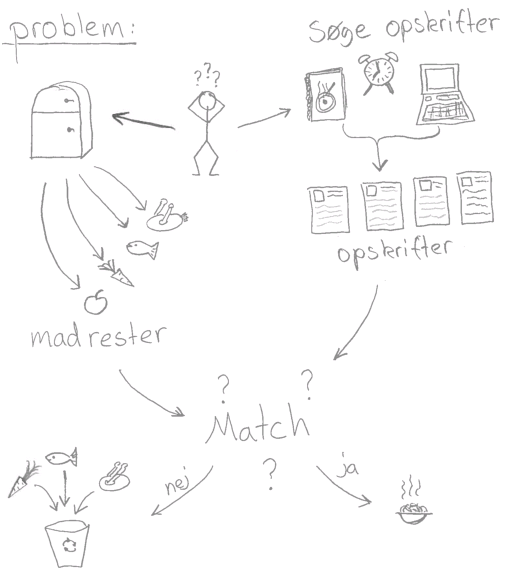
\includegraphics[scale=0.6]{billeder/rigebilleder/problemomraade.png}
\capt{Rigt billede, der visualiserer problemet ved at skulle genbruge madrester.}
\label{fig:rigbillede1}
\end{figure}

Det rige billede i \figref{fig:rigbillede1} viser en bruger, der ikke har tid eller ressourcer til at finde ud af, hvordan madresterne, der er i køleskabet, kan blive brugt i madlavningen. Det rige billede har hjulpet os til at få en forståelse for situationen.

%afslutning
På baggrund af samtalerne med informanterne, skal vi udarbejde systemdefinitioner og udvælge en af disse, som vi skal basere vores videre arbejde på. For at være i stand til at udarbejde systemdefinitioner effektivt, har vi valgt at undersøge nogle eksisterende systemer, der forsøger at løse en lignende problemstilling, som den vi arbejder med.